\section{Stuck in Paradise}


\margininbox{Stuck in Paradise}{
     \begin{itemize}
    \item Gergely Ambrus
    \item Jana Čarga
    \end{itemize}}{\explo}

It is always nice going caving with Jana. Good mood, good stories, good
food and good zganje, what else do you need? :) So, as soon as we had a
slot for going to the underground camp, we made use of it. The only
question was: where to go? The first day we checked out some
possibilities close to camp, but none of them seemed to be super
exciting.

At camp we had a jolly time: Clare and Tetley were with us on the day
train, while Jarv and Dan pushed on the night train. Tetley and Clare
pushed \passage{Amazing Grace} to \passage{Magic Dragon}, and they were very
excited by what may lay ahead. So Jarv and Dan went to check that out.


\begin{pagefigure}
\checkoddpage \ifoddpage \forcerectofloat \else \forceversofloat \fi
   \centering
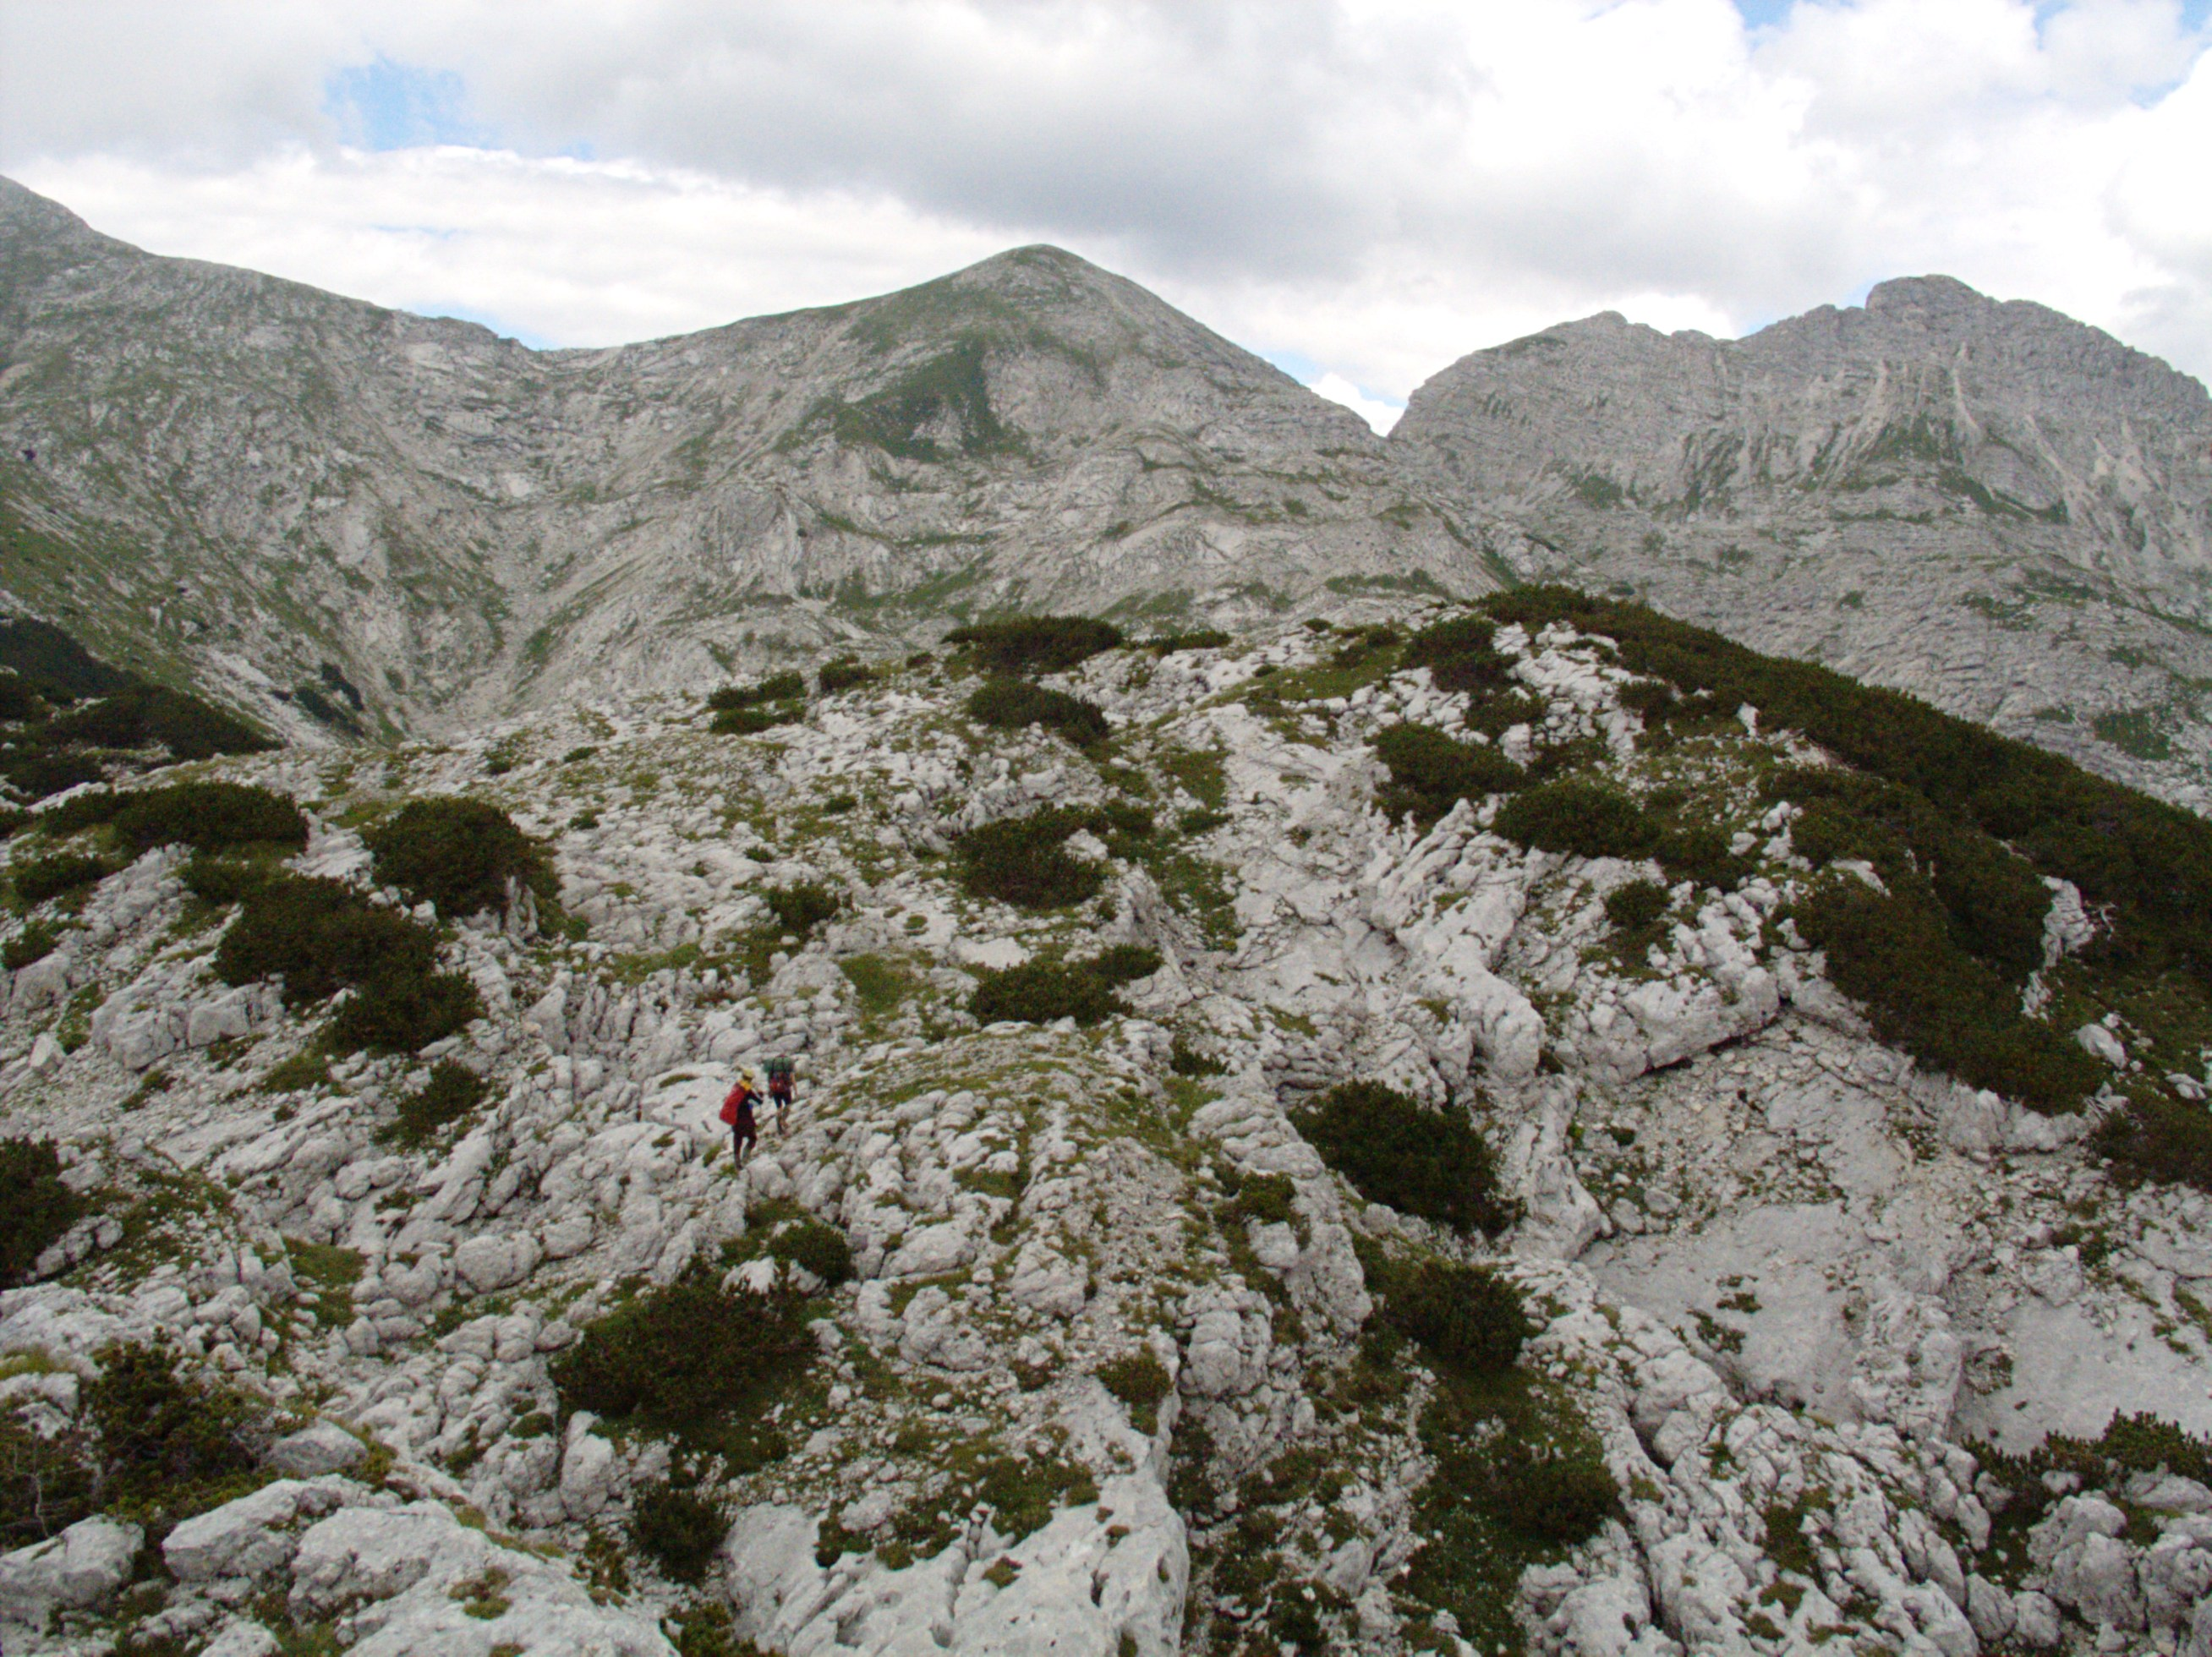
\includegraphics[width = \textwidth]{2011/stuck_in_paradise/2011-07-29-12.19.20-Jarvist Frost-CanonG5-CRW_0118 - Jana and Gergely off to underground camp heading towards M2--orig.jpg}
\caption{Jana and Gergely crossing the stunning scenery of the limestone plateau of \passage[mountain]{Migovec} to reach \passage{Vrtnarija}, passing hundreds of holes on the way, including the entrance of \passage{M2}. \pic{Jarvist Frost}} \label{jana gergely cross plateau}
\end{pagefigure}

In the morning, good news arrived with Jarv and Dan! A large pitch
waiting for us, said Jarv, very welcoming, exciting, and\ldots{} muddy.
So muddy that they had no idea even about how to start rigging it, plus
they ran out of time too, so it is waiting for us! Well well, of course
we like challenges, and challenges like us too, so why not going there?

\margininbox{30-7-11 23:58}{
Yesterday we visited \passage{Magic Dragon} -- nice crystals/quartz.
Degraded rather horrifically after PSS.1 ; we started to bolt the pitch
but the rock was appalling. Broken \& soft, quartzite broke the Spitz
teeth. Got a bolt in \& natural back up, went over the edge in the
horrific muddiness. The obv natural over the edge turned out to be mud. The whole pitch lip in fact sticky mud \& white cheesecake boulders. \name{Jarv}}{\logbook}

By then, the horizontal developments became very long, with several km
of passages. To get to the pitch, we needed about 2 hours of caving from
Camp \passage{X-Ray}. It was very nice to go there, to put together the
little pieces of information puzzles from the various teams, who all had
their share of exploration. It really was a team effort, and it really
was a victorious effort to find so many new places in this underground
chasm. So, we proceeded and thought along these lines, occasionally
fighting with super uncomfortable ropes, other times with super tight
squeezes, but yet, in general, being inspired by the cave -- such a
complex system!


\begin{pagefigure}
\checkoddpage \ifoddpage \forcerectofloat \else \forceversofloat \fi
   \centering
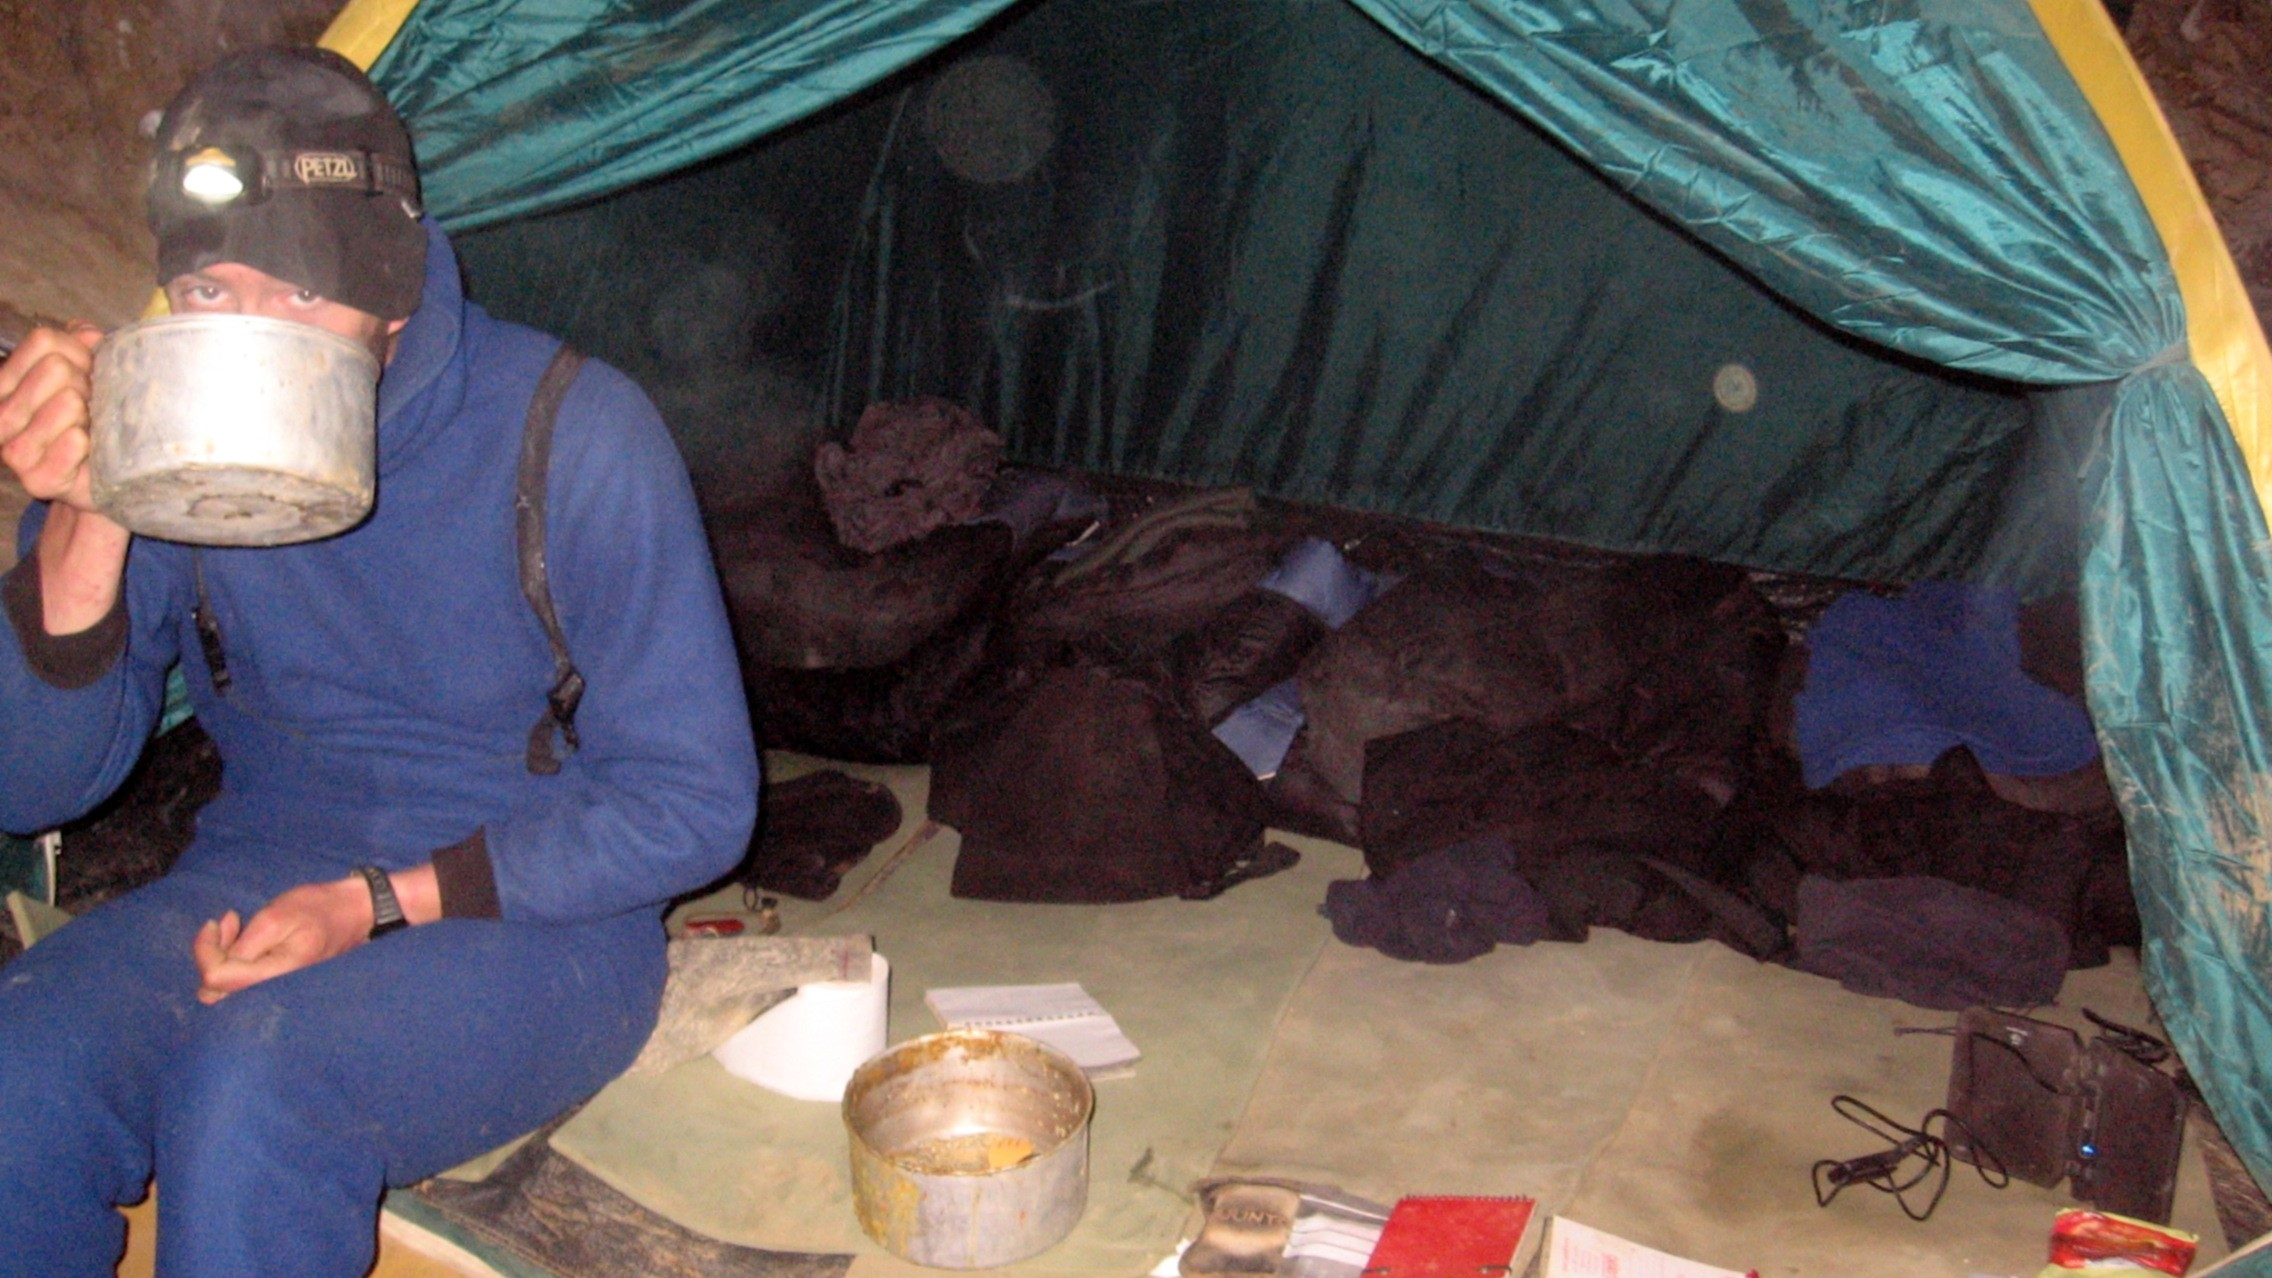
\includegraphics[width = \textwidth]{2011/stuck_in_paradise/2011-08-01-13.24.09-Jarvist M Frost-CanonA520-IMG_0173 - Dan Drinking Tea in the Tent at Camp X-Ray--orig.jpg}
\caption{Dan enjoying a brew at camp \passage{X-Ray}. \pic{Jarvist Frost}} \label{dan brew}
\end{pagefigure}


And then there we were. Up until about 50 meters before the pitch, it is a
nice, dry, sandy passage -- and then, this sea of mud appears beneath
your feet! We found the last PSS, had a look down, and then faced the
same problem as our forerunners -- how to start??

We thought that the wall on the left hand side seemed somewhat better,
so after a complex effort involving countless slips down, we managed to
get up there. The rock was quite OK, as soon as I removed the cca. 20 cm
of wet, sticky, disgusting mud covering it. So I started to bolt down,
and to build a nice rigging line -- the only bad thing being that nobody
can actually see that it is a nice line, because everything was covered
in so much mud. We were quite amazed when at the bottom, we looked at
each other -- all our SRT kit, tackle sacks, oversuits, and even our
faces, were basically just a big lump of mud. Well well, it is a good
idea to name the place\ldots{} Stuck in mud? But the name of the expo
was about Paradise, so why not call it \passage{Stuck in Paradise}? Bingo!
And thus, the name of one of the muddiest pitches within the mountain
was born!

At the bottom of the first chamber, we reached a rock bridge. Left or
right? We decided to check out the chamber on the left. We climbed up a
water inlet, which closed up at the top, and checked every possibility
-- concluding that indeed, the continuation is to the right. By that
time, we were running late, so we decided to leave the next part of
funny muddy rigging to another group (which happened to be Izi and me),
and surveyed back the pitch. We returned to camp a lot richer -- rich
with experiences, and even more rich with the amount of mud that covered
us!

\margininbox{31/7/11 11:17am}{Amazing two pushing trips with Tetley down \passage{Magic Dragon} and
\passage{Daydreamers} -- \passage{Vrtnarija} is now deeper than ever before!
Put in my first bolts and properly dropped first pitches; cheers Tet for
an incredible camping trip and great company. Top tip: hot brews at -800
m is the absolute dogs bollocks. \name{Clare}}{\logbook}


To top things off, the next day we went to do an easy pushing
project close to camp, that we named \passage{Lower Pleasures}. It was a muddy
dig, where we fought with one boulder for about 3 hours -- of course, at
the end we won! Behind the rock, another muddy pitch opened\ldots{} but
this waited for someone else. So, another nice trip, and a project to be
continued!

\name{Gergely Ambrus}



\fullwidthbox{The Rutars go pushing}{

\textit{1.8.2011 2100} -- Grega \& Tjaša. We are going down the stuff (\passage{Let na Drugi Svet}?) which found Samo and Izi. We did some digging and heard a loud water noise. There was a big draft. We came to water but we had no time to check its way (we leave it for next day probably). Night! \name{Tjaša}

\textit{2.8.2011 22:00} -- Nejc \& Karin. We came down around 4:00 had some tea and then we went to \passage{Lower Pleasures}. We tried to bolt it but we just couldn't. We came back and sleep. Nejc is sick so we're going out. There is some rope in \passage{Lower Pleasures} left (I think 2 pieces about 10-20 m long). \name{Karin}}


\fullwidthbox{1-8-11 Jarv and Dan}{

Yesterday we worked on the pitch below \passage{Longwater}. Didn't much like the
wet way pushed by Myles \& Mike \passage{Duffers Drop}, we went off \passage{Rotten Row}.

Suggestion to keep on rigging is to keep on deviating on left wall, then
bounce to right wall into continuation of rift for the final hang.

The Y-hang gives a perfect hang to the spray lashed ledge -- one could
just throw caution to the wind \& zip down, slam in a bolt in the wet
and continue.

The \passage{Rotten Row} PSS 1 was knocked off its corner, I hid the label in the
roof -- it sits on the little ledge on the right about halfway down the
traverse. \name{Jarv}}


\newpage

\section{Bolt climbing in The Queen's Bedchamber}

After a couple of days without caving, Gergely invited me to go camping
underground with him for he had a plan. The plan was to bolt climb the
aven at the end of the \passage{Queen's Bedchamber}. Therefore he packed a
large amount of equipment as he feared he might run out of gear during
the attempt. In the end we carried down a total of 3 tackle sacks.

\margininbox{Queen's Bedchamber}{
     \begin{itemize}
    \item Gergely Ambrus
    \item Iztok Možir
    \end{itemize}}{\explo}


Once in a camp we packed all necessary for bolt climbing. When we
arrived, I said to Gergely, "You start climbing first."

Gergely looked
at me and said: "I have never bolt climbed before, you go first."

I looked at him back and said: "Well, I have never bolt climbed before
either. I have always free climbed."

\begin{figure*}[t!]
\checkoddpage \ifoddpage \forcerectofloat \else \forceversofloat \fi
\centering
 \frame{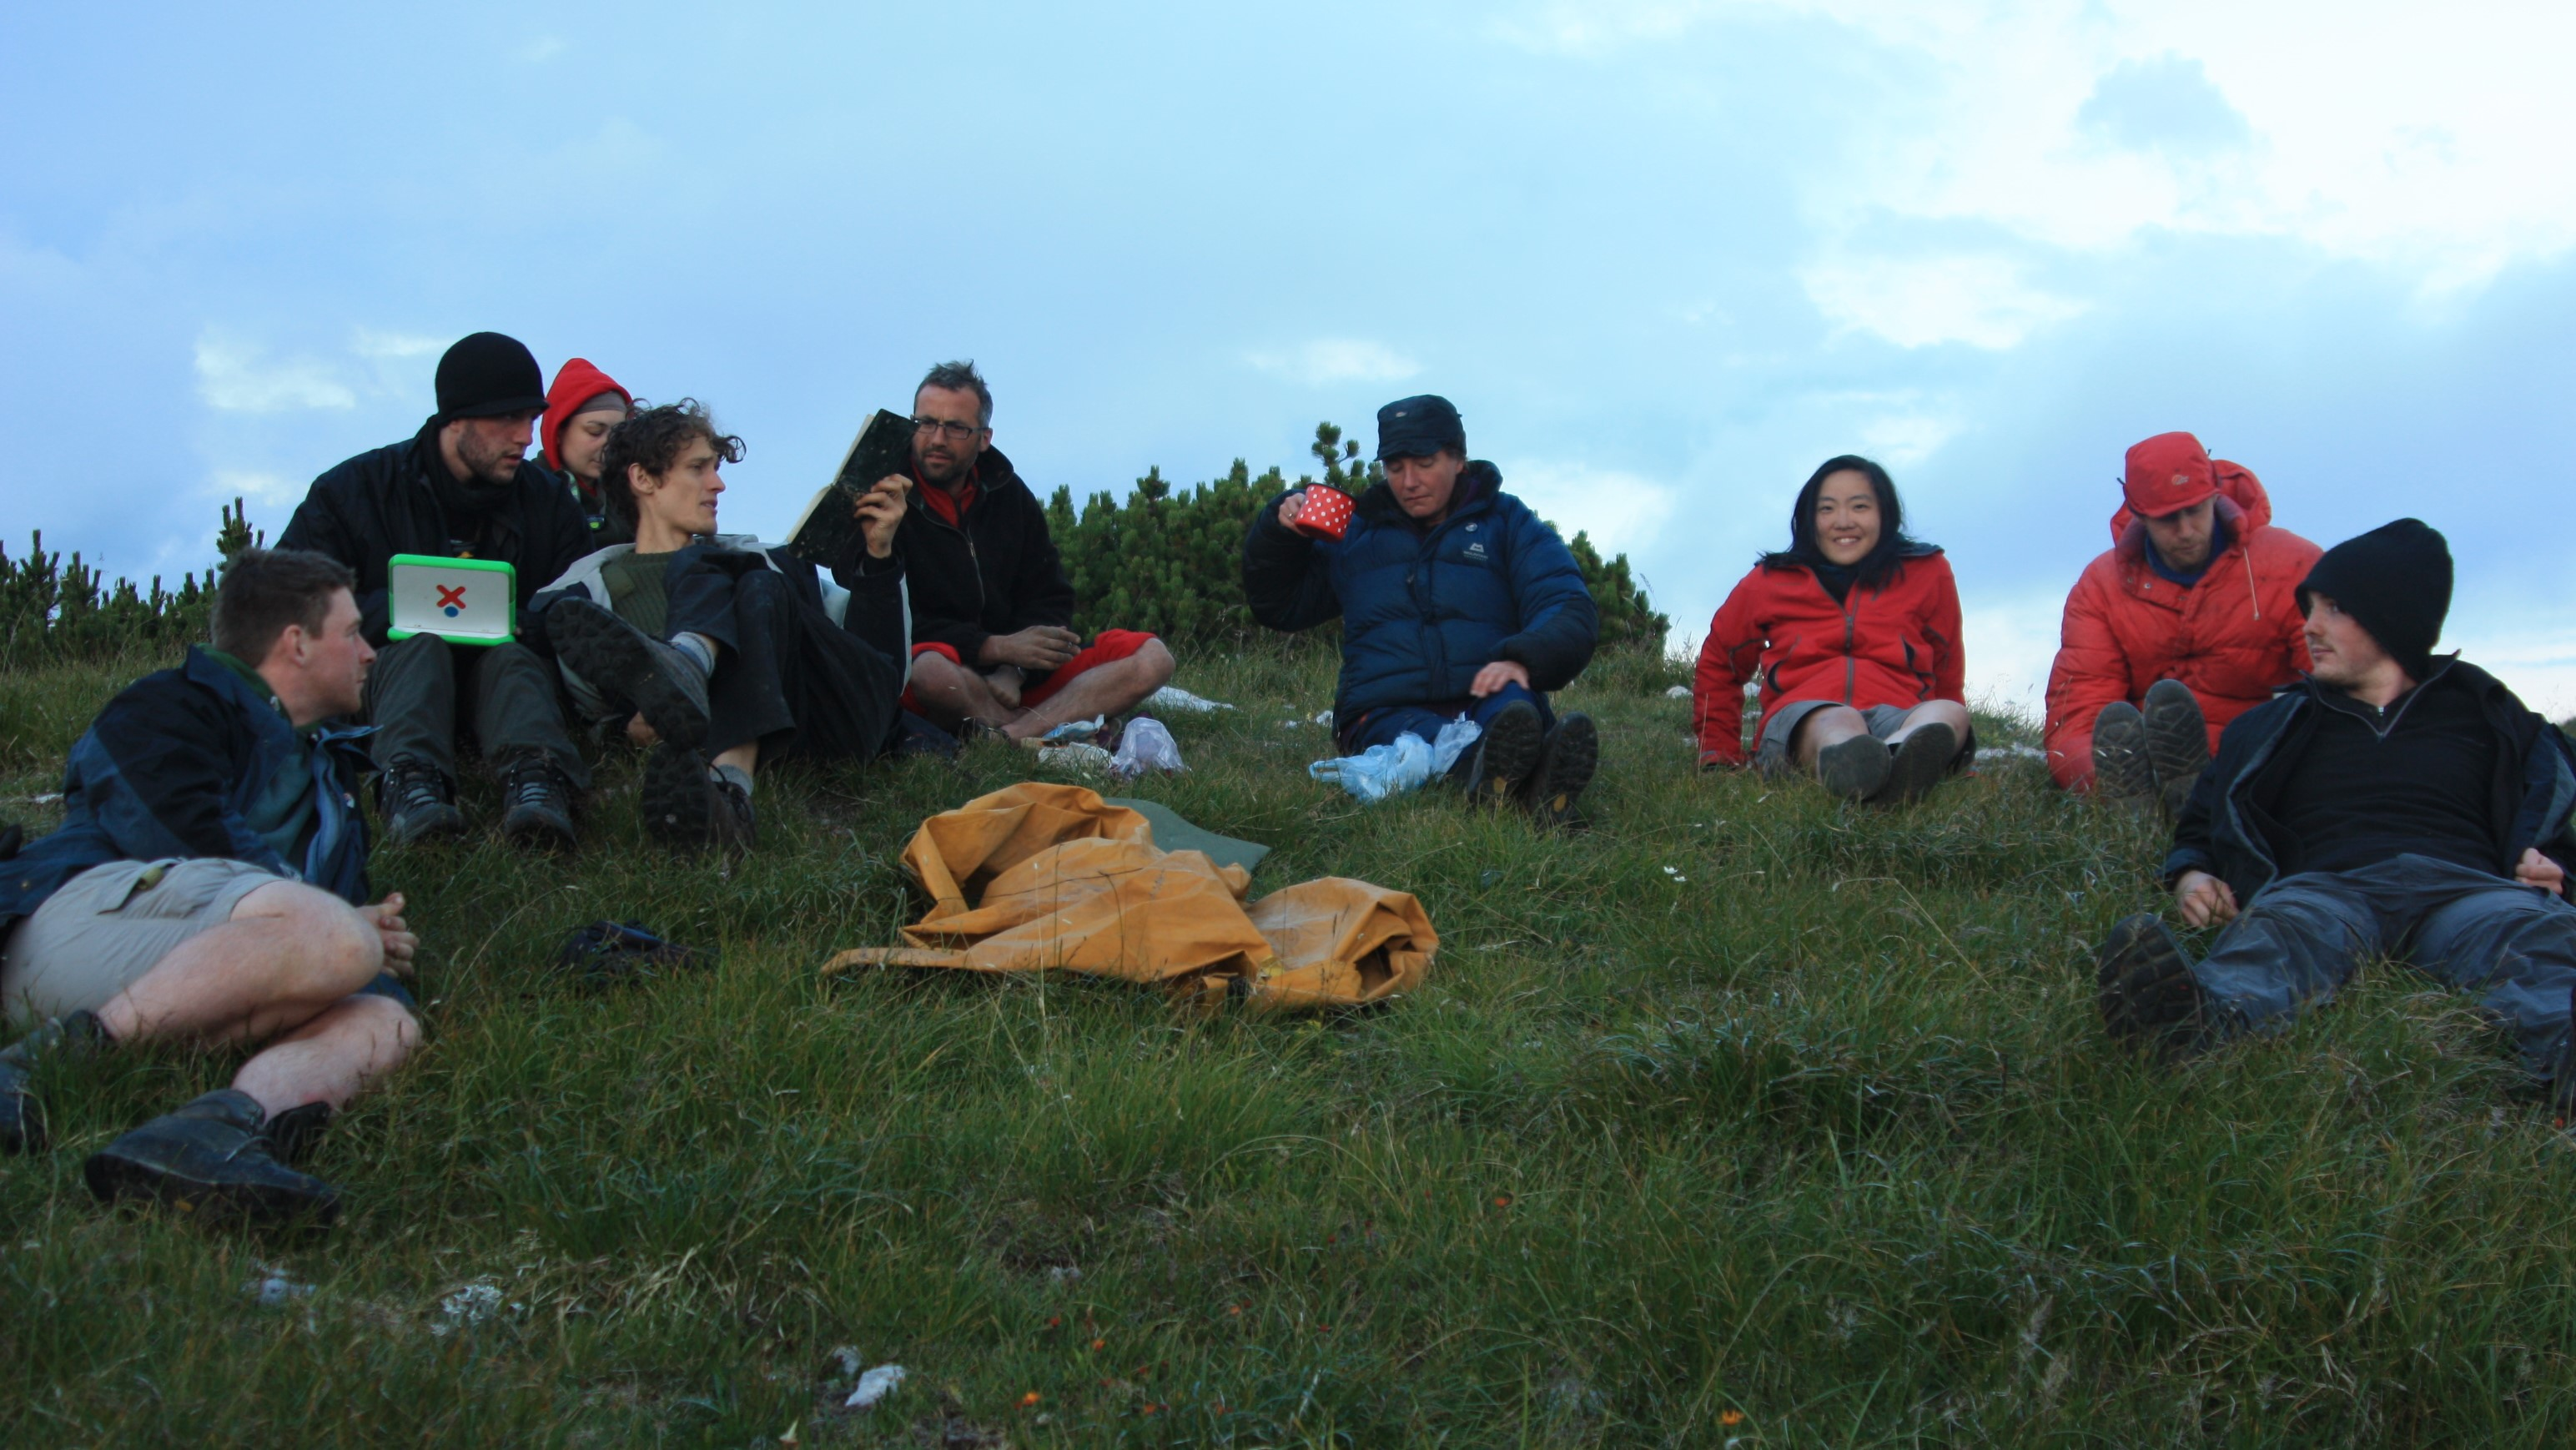
\includegraphics[width=\linewidth]{2011/stuck_in_paradise/2011-07-28-19.23.07-Gergely Ambrus-Canon450D-IMG_0735-Plateau--orig.jpg}} 
 \caption{Entering and studying survey data using the laptop at sunset spot. (The chill does not stop some from wearing shorts.) \pic{Gergely Ambrus}}
 \label{dan jarv data}
\end{figure*}

We start to laughing and decided that for sure can not be that hard and start to making a plan on how to do it. I started to bolt climb first, while Gergely was belaying me. After 9 m I was stopped by a big patch of mud. I tried to do the bolt above it, but was about 30 cm too short to drill a hole above the mud. At this point I decided that this is the end of climbing for today. I was climbing with a dynamic rope so what was left to do was to safely secure the static rope, till the point where I was able to reach.

\begin{marginfigure}
\checkoddpage \ifoddpage \forcerectofloat \else \forceversofloat \fi
\centering
 \frame{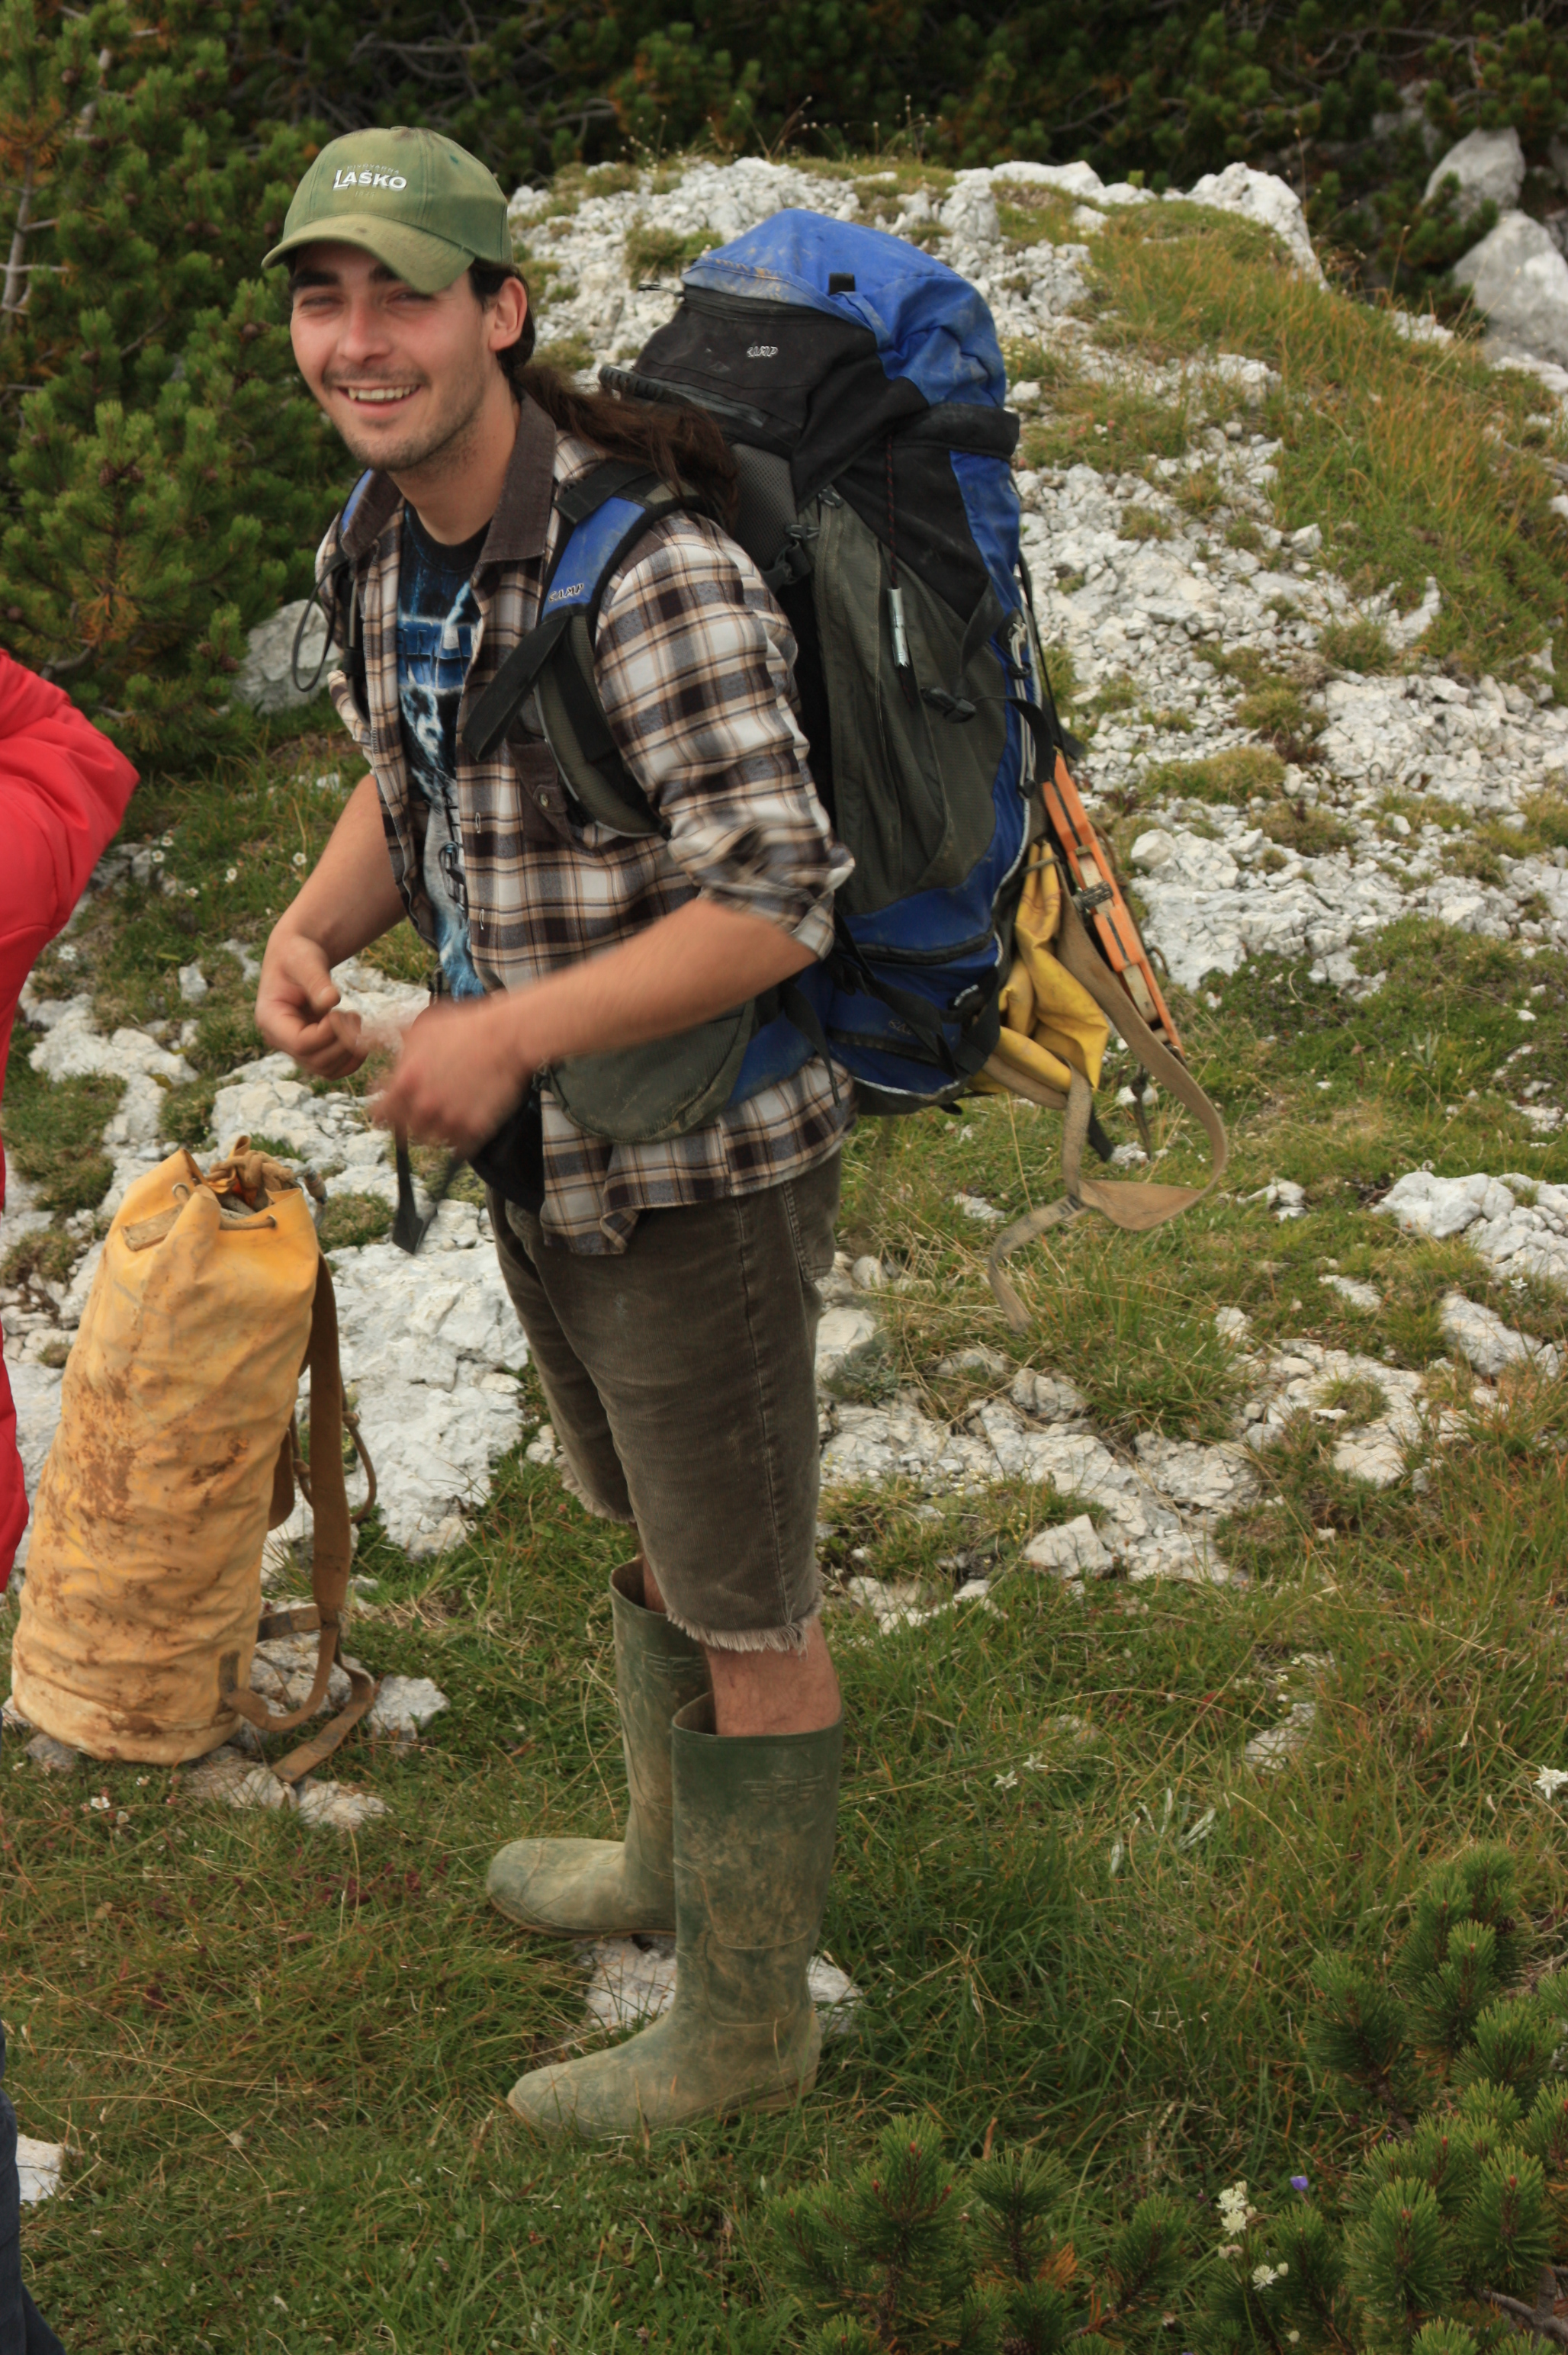
\includegraphics[width=\linewidth]{2011/stuck_in_paradise/2011-08-01-11.29.46-Gergely Ambrus-Canon450D-IMG_0781-Plateau--orig.jpg}} 
 \caption{Izi, ready to cave. \pic{Gergely Ambrus}}
 \label{izi ready}
\end{marginfigure}

Back to the camp, while eating we made plans for the next day. \name{Iztok Možir}


\section{The continuation of Stuck in Paradise}

\margininbox{Lost Miles (East Links)}{
     \begin{itemize}
    \item Gergely Ambrus
    \item Iztok Možir
    \end{itemize}}{\explo}

    
\margininbox{Penitence (Knee Killer)}{
     \begin{itemize}
    \item Gergely Ambrus
    \item Iztok Možir
    \end{itemize}}{\explo}


We started going towards \passage{Stuck in Paradise} to push this pitch
that Jana and Gergely had started bolting. On the way there, he was
explaining how big the pitch was, and how I would like it. When we
arrived there, it turned out he was right about the size of the pitch,
but he had not mentioned that it was full of mud.

As soon as Gergely was down with the drill on a bolting mission, I
started smoking and singing to myself. After an hour or so, Gergely
signalled that I could start descending. He made a hell of a rigging
effort, especially considering all the mud. Once we reached the bottom,
all the effort was paid off.

We were at the beginning of a horizontal gallery very similar to the
\passage{Palace of King Minos}. We followed the main passage all the way to
the end, where we were halted by a boulder choke. We tried to drill and
hammer our way through, but no luck there, so we decided to start
surveying back.

Because the passage was wide, it was fairly easy to survey. Soon we
reached the bottom of \passage{Stuck in Paradise}, but just a couple of
meters before we noticed that the draft actually went into a side
passage. We started crawling in this passage, which was tight all along;
after about 30 m we encountered another boulder choke.

\tweet{6:19PM Jul 29, 2011}{Well over 500m new now,another large rotation of underground campers this weekend.Weather finally pleasant ish, even saw stars last night!}

We noticed a possible way on through, but we decided to leave it for
some other team and surveyed back to the main passage, however it was
quite an effort. We named it \passage{Penitence}, because you had to crawl
on your knees for the most part and the main passage was named
\passage{Lost Miles}. All what was left to do was surveying \passage{Stuck in
Paradise} pitch itself. It ended up being quite a challenge as it was so
hard to read the instruments due to the amount of mud. In the end, we
connected everything with the P.S.S. at \passage{Magic Dragon}. Then it was
time for quick smoke, some pictures and the long return to camp
\passage{X-Ray}.

\name{Iztok Možir}

\section{How Miles of passage were lost!}

So, there was \passage{Stuck in Paradise}, left at the middle, and however
hard we tried to advertise it with Jana, nobody seemed to be quite keen
to go there and reach the kilometres of horizontal passages at the
bottom. Since it has been another example of truly Eastern European
cooperation, we decided to give it a go with Izi. I am always ashamed
when caving with him: he perfects minimalism, while I always tend to
pack too much of everything. This was not different this time either,
and \bignote{he looked amazed, and in disbelief, at the amount of food I had
prepared} for taking underground. So I discarded half of it, making sure
that the smoked meat, bacon and onion was making its way down to
underground camp -- it is so lovely to have a nice soup at camp full of
meat and fresh onion!



\begin{figure*}[t!]
\checkoddpage \ifoddpage \forcerectofloat \else \forceversofloat \fi
    \centering
        \frame{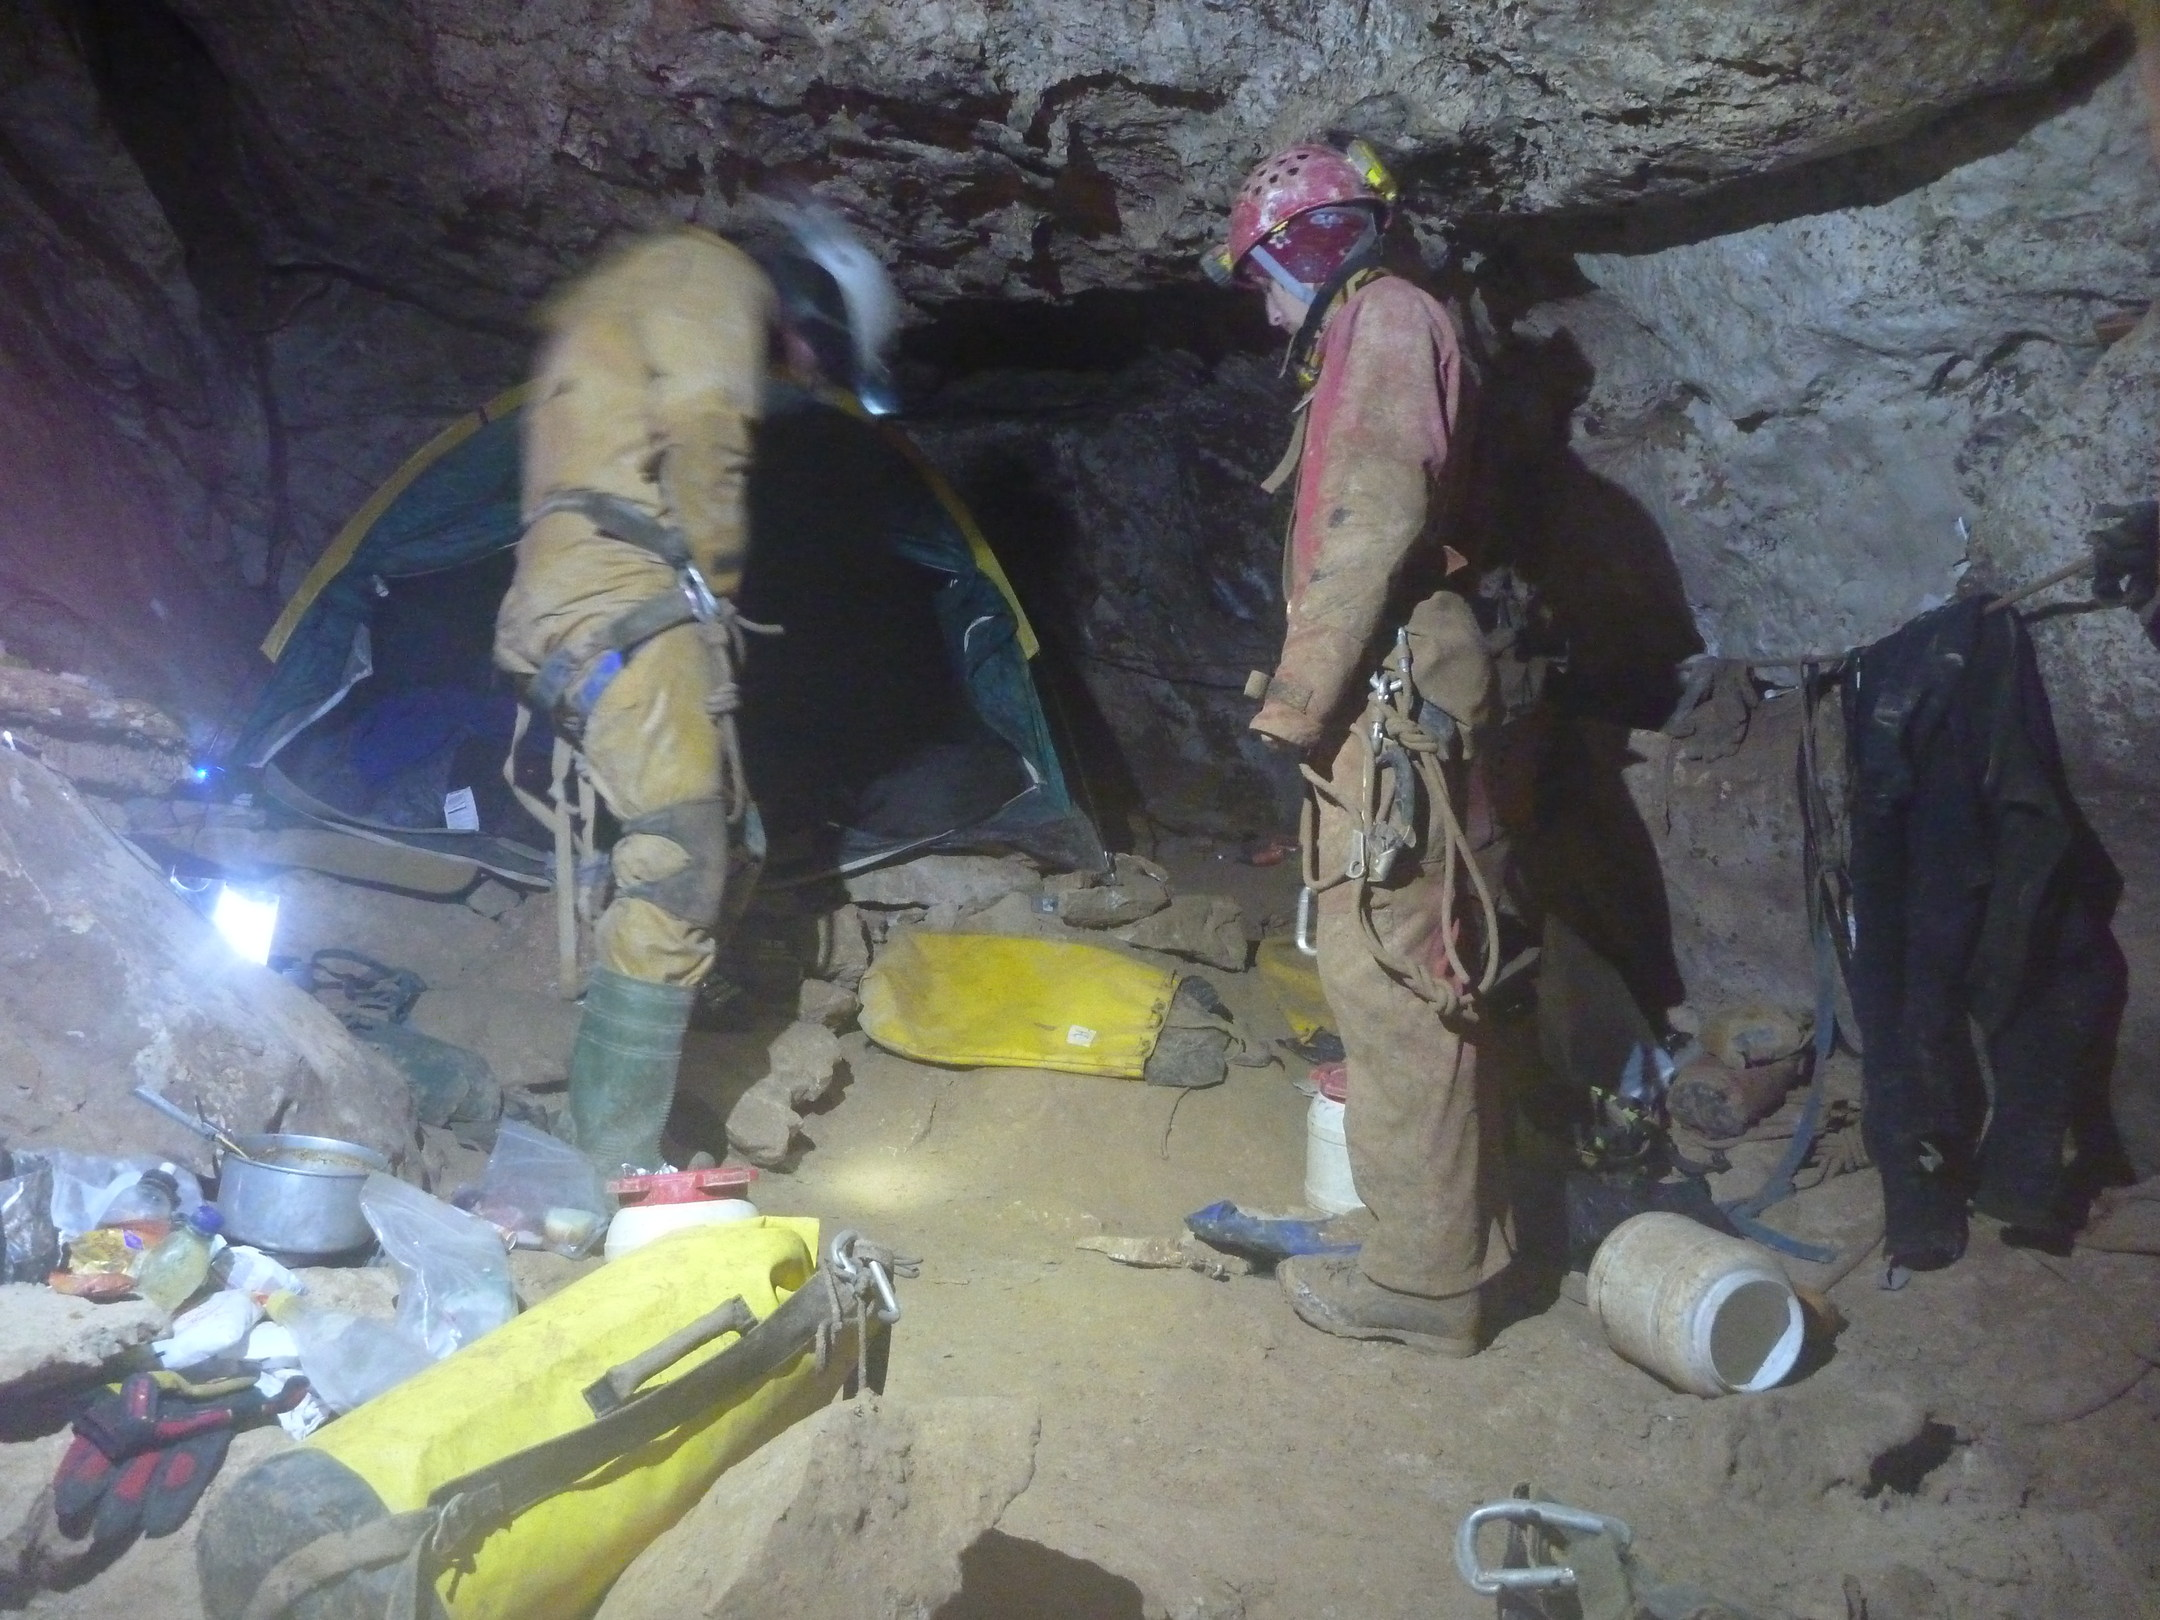
\includegraphics[width=\linewidth]{2011/stuck_in_paradise/2011-08-03-10.31.54-Grega-Panasonc DMC-FT2-105-camp x-ray--orig.jpg}} 
        \caption{Getting ready to go pushing from camp takes a little while, just like getting ready to go caving on the surface. \pic{Grega Maffi}} \label{prepping to push}
\end{figure*}


On our first day, we went to climb in the \passage{Queen's Bedchamber},
starting a long-term project. Then, the second day came our big task --
to continue \passage{Stuck in Paradise}.

We packed two batteries for the drill, plenty of rope, also a good
amount of food, so once again, we felt like being mules when reaching
the southern end of the cave. Nevertheless, we made good progress, and
soon I was on the rope again, continuing the rigging.

There was no surprise: mud and mud, but this time even spiced up with a
number of falling rocks. Hmm, what a nice combination! I tried to lead
the rope out of the fall-zone with more or less success. Meanwhile, poor
Izi was getting very cold at the rock bridge. Finally, the battery died,
so at last he had a chance to move. We joined our efforts to finish the
bolting, at the bottom of the pitch there was yet one more little drop
to do. Finally, we cut the rope, and started to see what lay in front of
us -- a horizontal phreatic gallery!

So, we started to proceed, with \bignote{Izi's goal: to break the record of the
longest new passage in one day}! Luckily, the cave seemed to be up to the
challenge: the tube went and went and went. We noted a passage on the
left, but continued first with the obvious gallery ahead. We found some
nice crystal-covered part, but apart from that, it was clear that
nothing serious happened to this ancient, old cave. It was in the same
pristine condition, as when the water left it, God knows when. It really
felt to be the most ancient part of the cave to me, very deep and far
from the entrance, \bignote{completely untouched for millennia}. So we went and
went, finally reaching a boulder choke. It cannot finish here! The only
tool we had with us was a bolting hammer, but nevertheless, we started
to work on it. At the beginning, it seemed completely blocked, but then
little by little, we gained more and more space between the boulders. It
was a nice puzzle, try to see where we might break through. Finally, we
were almost at the other side! However, the last rocks proved to be too
big for our bolting hammer, and we had to give up the work, knowing that
with a chisel it would take maybe half an hour to break through (which
indeed proved to be the case the next year). So, we started to survey
back -- we really liked to test the range of the Disto :) Then, when
reaching the junction, we had a look in the other passage. There was a
lot of draught here! Unfortunately, this proved to be much smaller than
the first tube, and the floor was filled with super uncomfortable little
stones. But, it contained the first real stalactites that I saw at \passage{Mig}!
We decided to named it \textbf{Knee-killer}, and the first passage
\textbf{East Links} (because we thought it was mainly going to east,
rather then south). Looking back at the names, it is obvious that we
were not at the height of our mental abilities! It has been a long trip,
maybe we were at the 16\(^{th}\) hour then.


\begin{marginfigure}
\checkoddpage \ifoddpage \forcerectofloat \else \forceversofloat \fi
\centering
 \frame{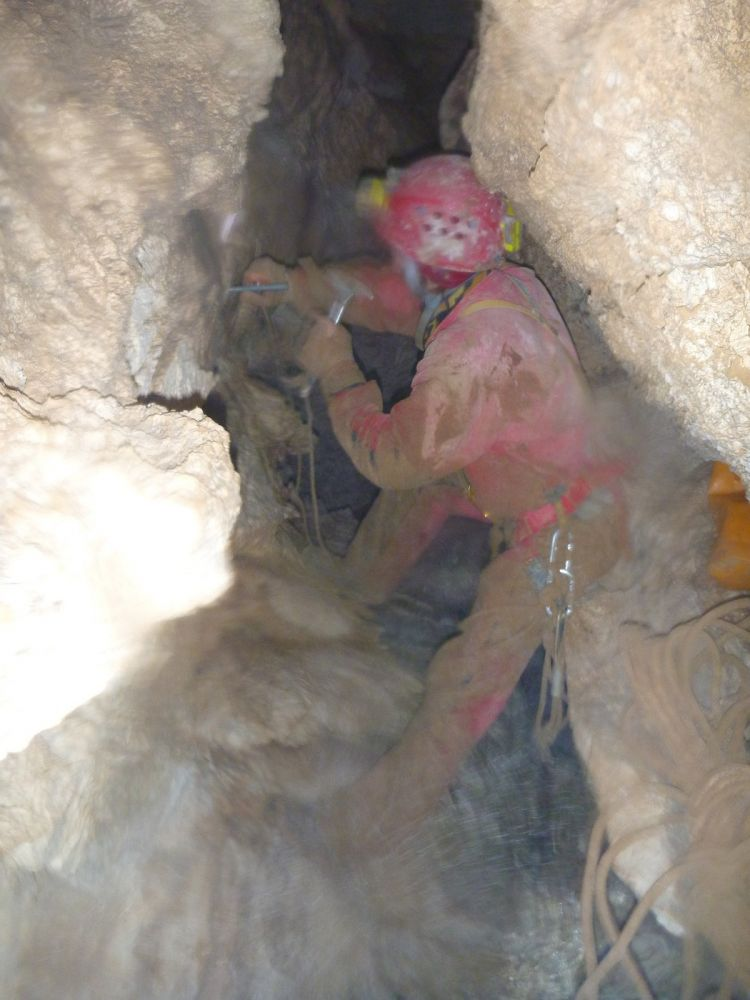
\includegraphics[width=\linewidth]{2011/stuck_in_paradise/2011-08-02-12.25.54-Grega-Panasonc DMC-FT2-102-Let Na Drugi Svet--orig_1050p.jpg}} 
 \caption{While Izi and Gergely were working in \passage{Stuck in Paradise}, Tjaša and Maffi continued to push \passage{Let na Drugi Svet}. \pic{Grega Maffi}}
 \label{tjasa bolt}
\end{marginfigure}

So, we were glad to find so much, but now we had to get back to camp! It
took ages prussiking up in \passage{Stuck in Paradise} for the first time,
really a nightmare. And after, numerous little squeezes, ropes,
traverses, to be topped by the ever fine experience of \passage{Cheetah} --
so, we were really exhausted when reaching the camp.

There was Tetley and Clare, and we started to tell him the news of
another Great Discovery! Our 40 m survey legs, the going leads, the big
pit\ldots{} all the great story! So, it was time to count the number of
meters we found that day -- Tetley asked to see the survey book of course.

``You have it, Izi,'' I said.

``No, it is in your pocket,'' came the answer.

``Maybe it is in the Daren drum?''

``Or with the bolting kit?''

``Or\ldots{}''

``Oh, F*ck!''

``Oh, Sh*te!''

Yes, indeed, it is true. We left it there. We could only hope that it was at the top of the pit, where we had a ciggy break, and not at the bottom.

So, the next morning, \bignote{we had to go back, completely broken}, again to
that marvellous place. Luckily, we found the survey book waiting for us
on the rock at the top of \passage{Stuck in Paradise}. Good lord! So, we found our
\passage{Lost Miles} again. And, right away, we also decided to replace our
crappy names by \passage{Lost Miles}, and \passage{Penitence}!

Did we manage to break the record? I don't quite know\ldots{} But it is
not important at all. We found a lot of passage (about 600 m), and the
mountain once again opened up a completely new part of the system. A
part, that later proved to be very interesting, fascinating, and
scary\ldots{}

\name{Gergely Ambrus}


After a good sleep, we were woken up by Tetley and Clare. On the way down to the camp, they had met another team, who had told them about our recent finds. As soon as Tetley saw us, he wanted to have a look at our survey book. I had been carrying it in my tackle bag, but when I wanted to show it to Tetley, I couldn't find it.

We started to panic after a little while, but then I realized that it had probably fallen out when we had stopped for a smoke in \passage{Magic Dragon}. We rushed back there and with huge relief found it. Back in the camp, I showed the survey book to Tetley. He immediately started to count the meters and then smiled to me and said: ``Yet again you've found more than 500 m, you are very lucky in your choice of caving partners.''

I replied: ``This is no luck, I only take the right people with me or they take me??'' After that, it was time to return to the surface for tea and medals.

\name{Iztok Možir}


\begin{pagefigure}
\checkoddpage \ifoddpage \forcerectofloat \else \forceversofloat \fi
   \centering
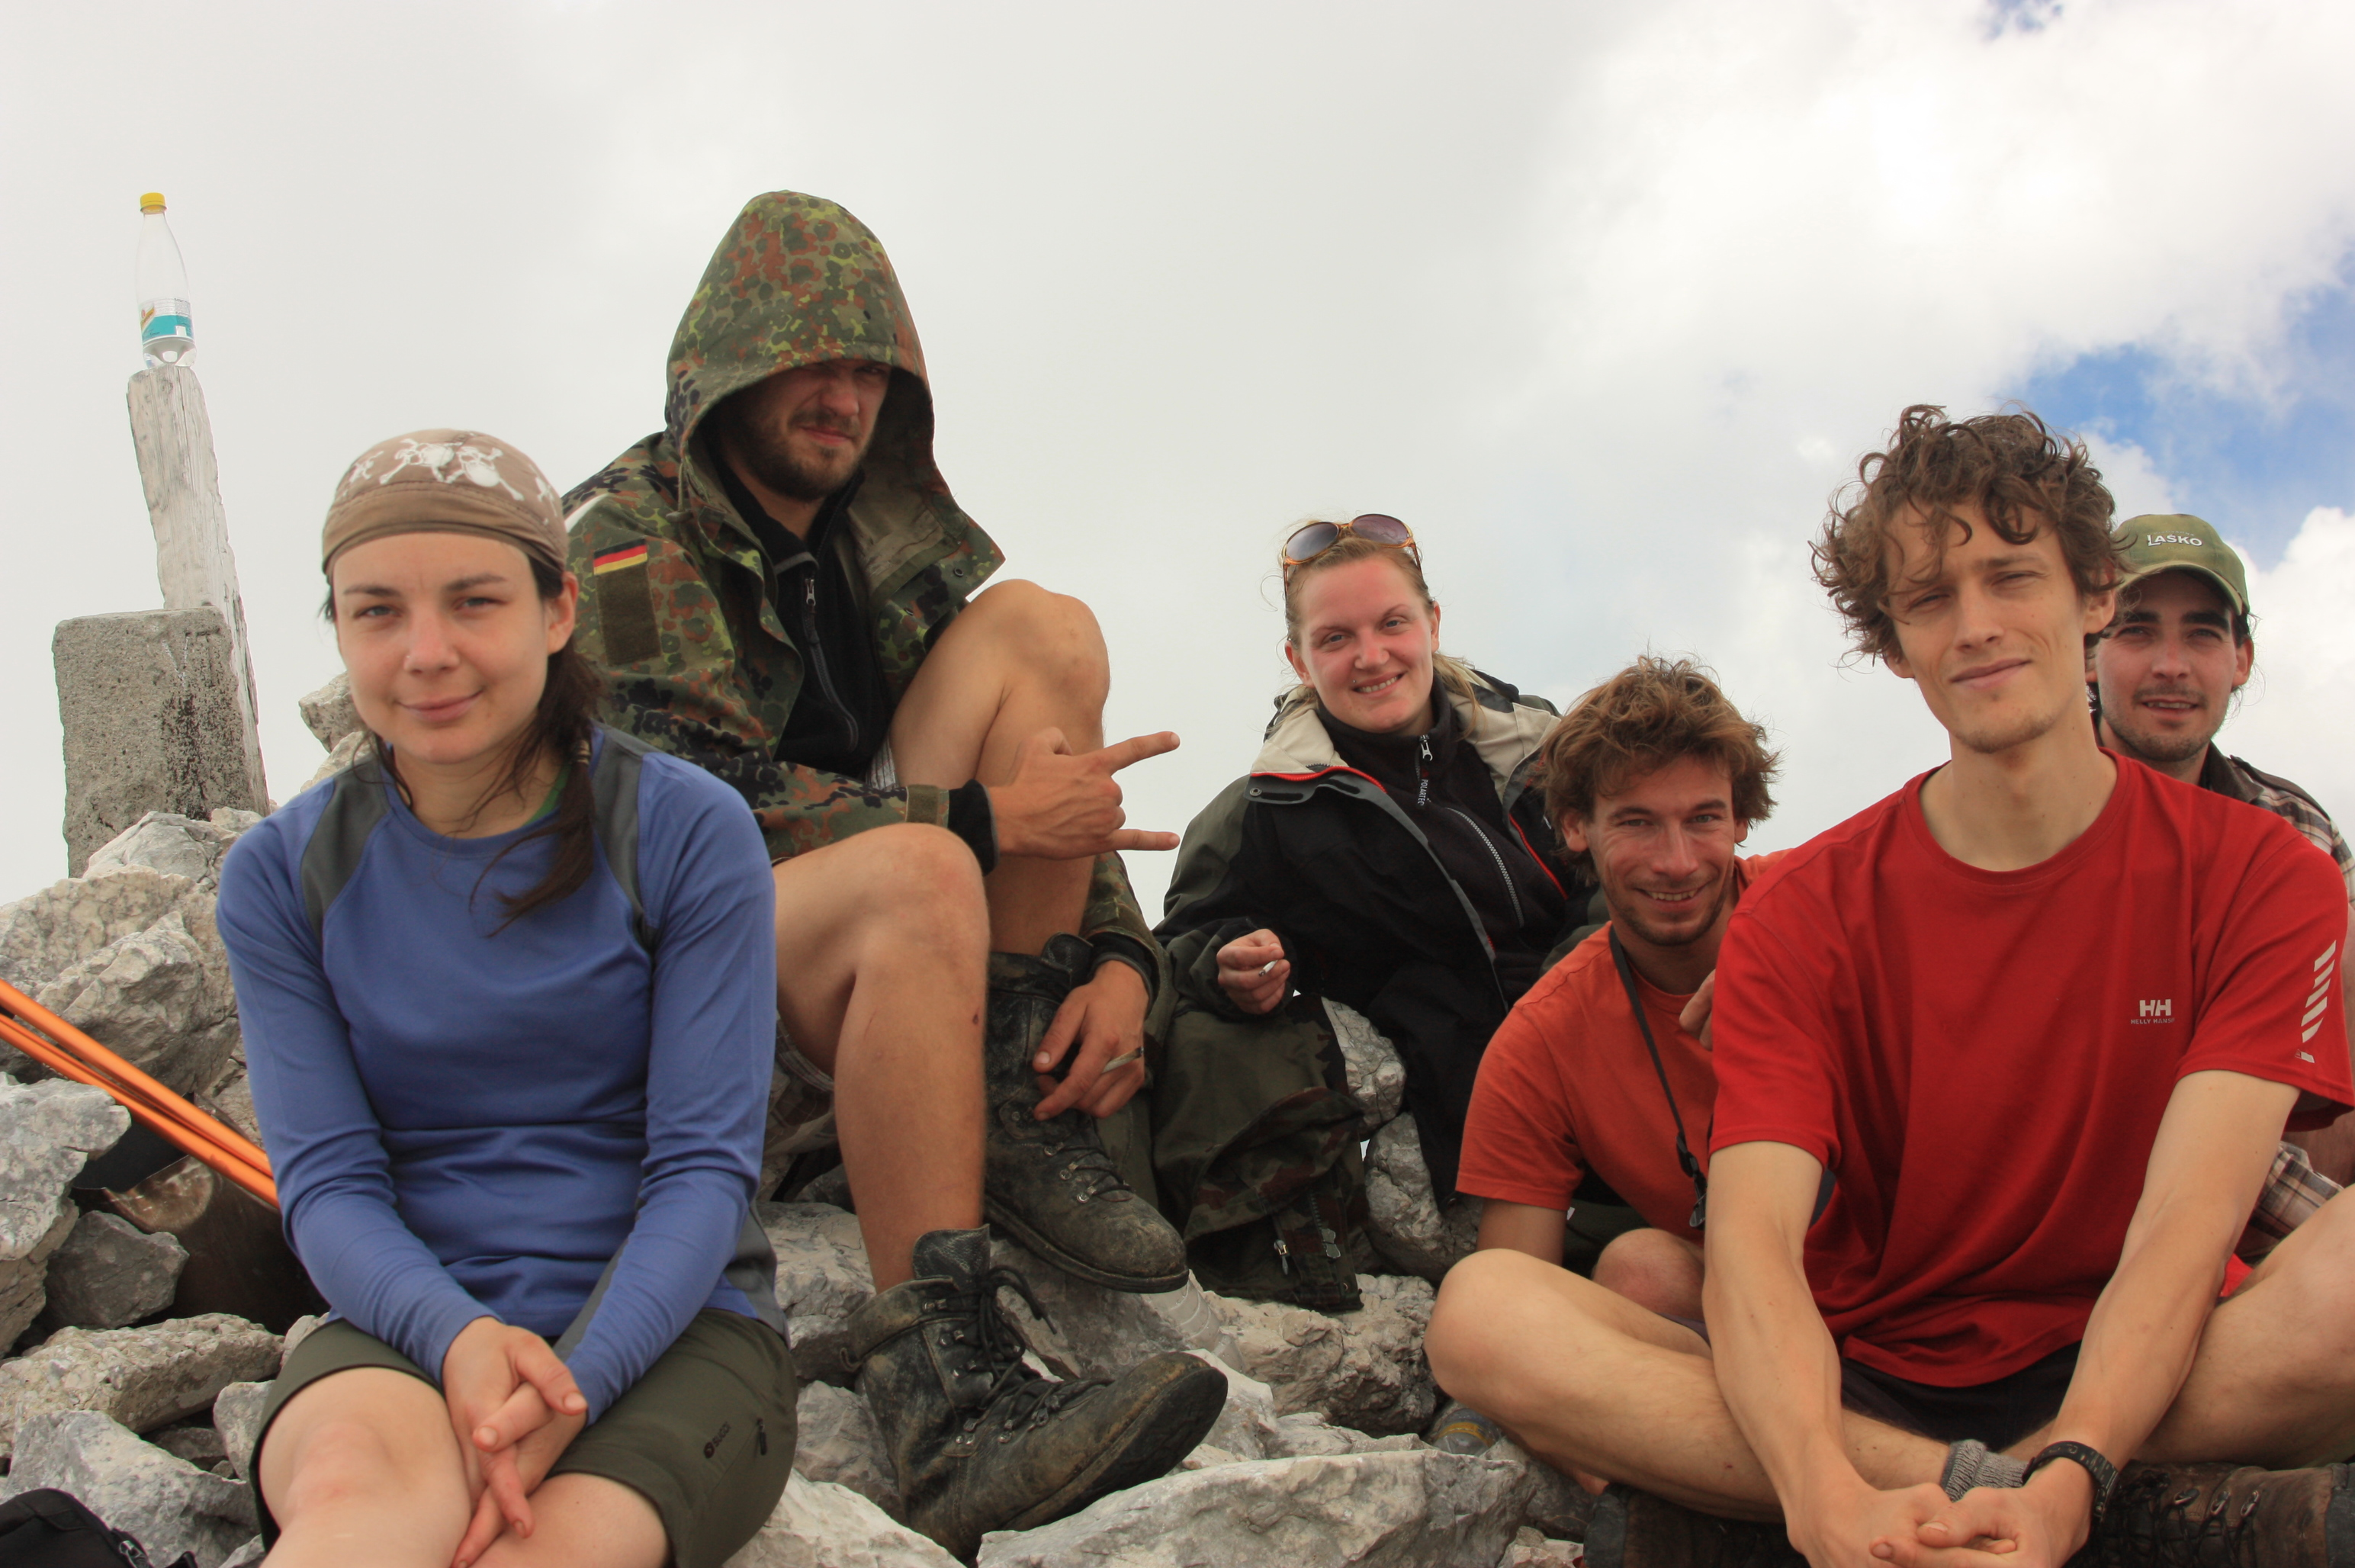
\includegraphics[width = \textwidth]{2011/stuck_in_paradise/2011-08-02-12.35.07-Gergely Ambrus-Canon450D-IMG_0854-Walk up Kuk--orig.jpg}
\caption{\textit{left to right} Jana, ??, ??, Gergely, Jarv and Izi at the summit of \passage[mountain]{Kuk}. \pic{Gergely Ambrus}} \label{kuk crew}
\end{pagefigure}
